% ---------------------------------------------------------------
% Shared body. Compiled by paper_ieee.tex (IEEEtran, for submission)
% and preview.tex (local two-column preview).
% ---------------------------------------------------------------
\begin{abstract}
Collaborative virtual reality (VR) is increasingly used for confidential enterprise meetings, yet access control in these spaces is usually a one-time login: whoever wears the headset afterwards inherits the avatar. We present \textsc{BoardroomXR}, a Unity system for Meta Quest that gates a shared virtual boardroom behind server-authoritative multi-factor authentication (PIN, 3D gesture, time-based one-time password) and then verifies the wearer \emph{continuously} from head and hand kinematics, revoking access and hiding confidential content when the motion stops matching an enrolled template. We ask whether such a verifier can reach an equal error rate (EER) below 5\%, and we answer with three kinds of evidence that we keep strictly apart. An idealised simulation of 40 synthetic users, executed through a verified port of the deployed code, gives a cross-session EER of 4.7\%. On the headset, the four authors recorded 11 sessions with templates cleared each time, deliberately moving differently in each session to stand in for different users. The entry gate worked well (11 of 11 owner gesture verifications passed at the first attempt; all 15 attempts on another author's gesture were rejected), and the continuous verifier locked out 9 of 9 deliberately induced behaviour changes, 7 of them within 2.5\,s of the first warning. However, the EER between different people was 17.2\% with interleaved test windows and 30.3\% with test windows from the end of the session. Body geometry separated people better (20.7\%) than motion dynamics (48.0\%), and a person's own, deliberately different session scored no higher than another person's (0.168 vs.\ 0.171). Much of this is posture: three authors recorded both seated and standing sessions, which moved their eye height by 30--50\,cm, more than the height difference between the authors when standing. A simulator re-calibrated to these statistics reproduces the observed lockout behaviour without being fitted to it and predicts that longer enrolment, geometry-only scoring and score averaging lower the EER to about 15\%, not to 5\%. We conclude that the 5\% target is met only under idealised conditions. The headset study involves four people and is a preliminary result; we report it as such and release the code, logs and simulators.
\end{abstract}

\begin{IEEEkeywords}
virtual reality, continuous authentication, behavioural biometrics, multi-factor authentication, head and hand kinematics, simulation
\end{IEEEkeywords}

\section{Introduction}
Head-mounted displays (HMDs) are moving from games into work: design reviews, training and executive meetings now take place in shared virtual rooms. These rooms inherit a weakness from desktop systems and add one of their own. Authentication happens once, at the door, and nothing checks afterwards who is actually wearing the headset. An unattended HMD can be picked up by a colleague, a visitor or an attacker, who then speaks, gestures and views confidential material as the original user's avatar. Interrupting the session with periodic explicit re-authentication would close the gap but breaks the presence that makes VR useful.

The motion of a person's head and hands carries identity. Prior work identified VR users from tracking data with high accuracy~\cite{pfeuffer2019,miller2020,nair2023} and used head movement for continuous authentication~\cite{mustafa2018,gyreyiri2025}. Most of these results come from offline classification of recorded datasets. Fewer papers describe what happens when such a verifier runs inside a live multi-user application on standalone hardware, behind a conventional login, while real people put the headset on and take it off.

This paper reports such a deployment and asks a concrete question: \emph{can continuous behavioural authentication from head and hand kinematics achieve an EER below 5\% against avatar identity spoofing in collaborative VR?} Our contributions are:
\begin{enumerate}[leftmargin=*,itemsep=1pt,topsep=2pt]
\item \textbf{A deployed design} that combines a server-authoritative three-factor entry gate with a lightweight continuous kinematic verifier, selectable operating points, an adaptive template and an explainable live trust display, all running on the headset (Sections~\ref{sec:design}--\ref{sec:impl}).
\item \textbf{A headset study} by the four authors (11 sessions with deliberately varied behaviour), preceded by a 14-session pilot, reporting the entry gate, the live verifier and offline error rates from on-device logs (Sections~\ref{sec:method}--\ref{sec:results}).
\item \textbf{A three-way comparison} of the same algorithm on idealised simulated users, on headset data and on a simulator re-calibrated to the headset data. The gap between the first two (4.7\% vs.\ 17.2--30.3\% EER) is the central result. The third reproduces the headset's operating-point behaviour, which it was not fitted to, and lets us test remedies at scale.
\item \textbf{Two negative results} with practical consequences: a speed-threshold anomaly detector of the kind often used as a first defence would have revoked 11 of 12 and 11 of 11 genuine enrolments in the two headset studies, and a deliberate change of movement made a person indistinguishable from someone else.
\end{enumerate}
We state throughout which numbers come from the headset and which from simulation.

\section{Related Work}
\textbf{Authentication in VR.} Knowledge-based schemes transferred from mobile devices (PIN, pattern) work in VR but are exposed to shoulder surfing and are slow to enter with a controller ray~\cite{george2017}. Stephenson et al.\ systematise AR/VR authentication and argue for schemes that exploit the sensors HMDs already have~\cite{stephenson2022}. Our entry gate deliberately uses conventional factors; our focus is what happens after it.

\textbf{Motion as identity.} Pfeuffer et al.\ identified users from head, hand and eye motion and the relations between body parts during VR tasks~\cite{pfeuffer2019}. Miller et al.\ identified 511 people with 95\% accuracy from less than five minutes of tracking data each, recorded while they watched 360$^{\circ}$ video~\cite{miller2020}, and Nair et al.\ scaled identification to more than 50{,}000 users of a commercial VR application~\cite{nair2023}. Li et al.\ authenticated smart-glasses wearers from head movement in response to audio stimuli~\cite{li2016}. These works establish that the signal exists, mostly for closed-set identification offline and often during a fixed task.

\textbf{Continuous authentication.} Mustafa et al.\ authenticated VR users continuously from head and body movement during free use~\cite{mustafa2018}, and Gyreyiri and Shukla studied head-movement biometrics for continuous authentication in VR~\cite{gyreyiri2025}. Miller et al.\ showed that motion-based verification degrades across days~\cite{miller2022}. Robustness to adversarial and real-world disturbances is studied by Chen et al.~\cite{chen2024}, and Li et al.\ show that motion forecasting can attack behaviour-based VR authentication~\cite{li2026}. We target the handover and stolen-credential threats and report how the verifier behaves inside a live system.

\section{Threat Model}
\label{sec:threat}
An enterprise runs a collaborative VR meeting in which confidential content (in our scene, a whiteboard) is visible only to verified participants. The legitimate user $U$ authenticates at session start. The adversary $A$ gains physical access to $U$'s headset during the session (it is put down, handed over or taken) and continues as $U$'s avatar, or logs in with $U$'s identity using credentials obtained by observation. $A$ may know $U$'s PIN and may hold the OTP token. Deliberate imitation of $U$'s motion is supported by the system as a demonstration scenario but is not evaluated here. The server is trusted; the client is not, so every verification decision is made on the host.

\section{System Design}
\label{sec:design}
\begin{figure}[t]
\centering
\resizebox{\columnwidth}{!}{%
\begin{tikzpicture}[font=\scriptsize, node distance=3mm,
  box/.style={draw=black!70, rounded corners=1.5pt, align=center, minimum height=6.5mm, inner sep=2pt, fill=#1},
  box/.default=white, >=Stealth]
\node[box=blue!6, minimum width=19mm] (pin) {PIN\\(salted SHA-256)};
\node[box=blue!6, minimum width=19mm, right=2mm of pin] (ges) {3D gesture\\(3-stroke template)};
\node[box=blue!6, minimum width=19mm, right=2mm of ges] (otp) {TOTP\\(RFC 6238 style)};
\node[draw=black!40, dashed, rounded corners=2pt, fit=(pin)(ges)(otp), inner sep=2.5mm, label={[font=\scriptsize\bfseries]above:Stage 1: entry gate (server-authoritative)}] (gate) {};
\node[box=orange!8, minimum width=40mm, below=7mm of ges] (feat) {head + 2 controllers, 6-DoF @ 60\,Hz\\3\,s windows every 0.5\,s $\rightarrow$ 16 features};
\node[box=orange!8, minimum width=27mm, anchor=north] (tpl) at ([xshift=-16mm,yshift=-5mm]feat.south) {enrolment: 60\,s\\template $(\mu,\sigma)$, adaptive};
\node[box=orange!8, minimum width=27mm, anchor=north] (score) at ([xshift=16mm,yshift=-5mm]feat.south) {$S=\exp(-\tfrac12 \overline{z^2})$\\EMA, preset $(\theta,k)$};
\node[draw=black!40, dashed, rounded corners=2pt, fit=(feat)(tpl)(score), inner sep=2.5mm, label={[font=\scriptsize\bfseries]below:Stage 2: continuous behavioural verification}] (cont) {};
\node[box=red!7, right=4mm of cont.east, anchor=west, minimum width=16mm] (rev) {revoke\\hide content\\restart MFA};
\draw[->] (gate.south) -- node[right,font=\tiny]{verified} (feat.north);
\draw[->] (tpl.north |- feat.south) -- (tpl.north);
\draw[->] (score.north |- feat.south) -- (score.north);
\draw[->] (tpl.east) -- (score.west);
\draw[->] (score.east) -| (rev.south);
\draw[->, dashed] (rev.north) |- (gate.east);
\end{tikzpicture}}
\caption{BoardroomXR architecture. All factor checks and the continuous verification decision run on the host; a revoke hides gated content for that avatar and restarts the entry gate.}
\label{fig:arch}
\end{figure}

\subsection{Stage 1: entry gate}
Fig.~\ref{fig:arch} summarises the design. A user first selects a virtual employee badge, which sets the claimed identity, and then completes three factors with the controllers. The \emph{PIN} is checked against a salted SHA-256 hash provisioned on the host. The \emph{gesture} is a 3D stroke drawn while the trigger is held, resampled to 64 points, normalised and compared with the enrolled strokes. Following the pilot (Section~\ref{sec:results}), enrolment takes three strokes; the second and third must reach a similarity of 0.5 with the first, verification takes the best match over the three samples, and the acceptance threshold is 0.65. Strokes shorter than 0.25\,s or 12 points are discarded as accidental. The \emph{one-time password} is a 6-digit, 30\,s time-based code shown on a virtual token and recomputed independently on the host. Only the host may set an avatar's \texttt{IsVerified} flag; an access gate hides confidential renderers until it does.

\subsection{Stage 2: continuous behavioural verification}
After the gate passes, the host samples the head (camera) and both controllers at 60\,Hz. Every 0.5\,s a window of the last $W{=}3$\,s is reduced to a feature vector $\mathbf{f}\in\mathbb{R}^{16}$ (Table~\ref{tab:features}): first-order dynamics (mean and standard deviation of head speed, head angular velocity and each controller's speed), higher-order head dynamics (mean acceleration and jerk magnitude), and body geometry and posture (mean head-to-controller distances and their spread, eye height, head pitch and inter-controller span). We call the first ten features \emph{dynamics} and the last six \emph{geometry}.

\begin{table}[t]
\caption{The 16 kinematic features computed per 3\,s window.}
\label{tab:features}
\centering\footnotesize
\setlength{\tabcolsep}{3pt}
\resizebox{\columnwidth}{!}{\begin{tabular}{@{}lll@{}}
\toprule
Group & Features & Unit\\
\midrule
Dynamics (10) & head speed $\mu,\sigma$; ang.\ velocity $\mu,\sigma$; accel.; jerk; & m/s, $^{\circ}$/s, m/s$^2$, m/s$^3$\\
 & R and L controller speed $\mu,\sigma$ & m/s\\
Geometry (6) & head--R dist.\ $\mu,\sigma$; head--L dist.; eye height; & m\\
 & head pitch $\mu$; controller span $\mu$ & $^{\circ}$, m\\
\bottomrule
\end{tabular}}
\end{table}

\textbf{Enrolment.} The first 60\,s after the first login produce 114 windows. The template stores the per-feature mean $\mu_i$ and standard deviation $\sigma_i$, with $\sigma_i$ floored at $\max(a_i, 0.02|\mu_i|)$ for a per-feature absolute floor $a_i$, so that a feature that barely varied during enrolment cannot turn millimetre noise into a large deviation.

\textbf{Scoring.} A full $16{\times}16$ covariance is poorly conditioned from about 100 overlapping windows, so we use a diagonal Mahalanobis distance:
\begin{equation}
z_i=\mathrm{clip}\!\left(\frac{f_i-\mu_i}{\sigma_i},\,-6,\,6\right),\qquad S=\exp\!\Big(-\frac{1}{2}\cdot\frac{1}{16}\sum_{i=1}^{16} z_i^2\Big),
\end{equation}
so that $S\in(0,1]$ and $S{=}1$ for a window identical to the template mean.

\textbf{Decision.} Raw scores are smoothed with an exponential moving average $\tilde S_t=\alpha S_t+(1-\alpha)\tilde S_{t-1}$, $\alpha{=}0.35$. A window with $\tilde S_t<\theta$ is a violation, and $k$ consecutive violations trigger a lockout, which revokes \texttt{IsVerified}, hides gated content and restarts the entry gate. The first deployment used $\theta{=}0.25$, $k{=}4$. Informed by the simulation in Section~\ref{sec:results}, the current build offers three presets selectable at run time: \emph{Strict} ($0.25$, $4$), \emph{Balanced} ($0.15$, $6$, the default) and \emph{Relaxed} ($0.10$, $8$).

\textbf{Adaptation and explanation.} While a user is verified with $S\geq0.6$, each template mean is updated by an exponential moving average ($\alpha{=}0.01$) for features with $|z_i|<2$; the update never runs in a warning or locked state, so an impostor cannot train the template. For each window the system ranks the features by $|z_i|$ and translates the largest deviations into plain-language reasons (for example, ``eye height 11\,cm lower than the enrolled profile''). These reasons, a live score graph and an event log are shown on a world-space panel, on a wrist display and on a laptop dashboard served by the headset.

\section{Implementation}
\label{sec:impl}
BoardroomXR is built in Unity 6 (6000.5.4f1) with the XR Interaction Toolkit and Netcode for GameObjects, targeting Meta Quest (Android, IL2CPP, arm64). The headset runs as host, so verification decisions are local to the authoritative process. The biometric module bootstraps itself at scene load, discovers the camera and controller transforms, and writes every scored window (state, raw and smoothed score, 16 features) both to a CSV file and to the system log, so data survive even if file retrieval fails. Structured event lines record every factor result, enrolment, lockout, preset change and identity switch. The study build adds six selectable employee badges, so several people can enrol on one headset, a procedurally generated boardroom with security doors that close on lockout, and audio cues. An earlier build also contained a \emph{speed-threshold anomaly detector} that flags head speeds more than 2.5 standard deviations from a rolling 1.8\,s baseline and revokes after three strikes; in the study build it only logs what it would have done. Fifteen Unity PlayMode tests exercise the real scene end to end, including complete logins through the keypad, enrolment of a scripted mover, a swap to a different mover, and lockout, content hiding and restart of the entry gate.

\section{Evaluation Method}
\label{sec:method}
\subsection{Pilot (first build)}
We first installed an instrumented build ($\theta{=}0.25$, $k{=}4$, single-stroke gesture at 0.75, legacy detector active) on a Meta Quest. Members of the project team took turns to log in, move naturally for a 60\,s enrolment, use the room and hand the headset to the next person without logging out. The pilot comprised 14 application sessions.

\subsection{Team study (study build)}
One day later, the four authors (P01--P04) used the study build on a Meta Quest~2 with the Balanced preset and a 60\,s enrolment, in 11 sessions (S01--S11; three, three, three and two sessions per author). Before each session all templates were cleared. In each session the author selected a badge, completed PIN, gesture enrolment and verification, and OTP, and then used the room while deliberately moving differently from their previous sessions, so that each session would stand in for a different user. At the end of most sessions the author deliberately changed the way they moved to test whether the verifier would lock them out. A laptop script captured the system log continuously and copied all files from the headset every 60\,s. Because every session was a fresh enrolment, a session acts as an identity for the live system; in the offline analysis we know which author produced each session and count only sessions of \emph{different} authors as impostors. This is a team study with four people, not a study of independent users; we treat it as preliminary evidence.

\subsection{Offline analysis of headset data}
Each complete session logged its 114 enrolment windows with all features, so we re-score them with a Python port of the deployed feature, template, scoring and decision code. The port reproduces the scores logged on the headset to within $5.5\times10^{-5}$ in the five sessions in which the adaptive template never updated; in the other six it had absorbed 2--43 windows before the lockout, so the logged scores differ slightly from a fixed template. We use three protocols. \emph{Held-out end (A):} the template is built from the first 68 windows (about 36\,s); the genuine test set is the last 40 windows, starting 3\,s later so that no window overlaps the template; impostor windows are the same 40 windows of every session recorded by a different author. This is the realistic case, because a template is always used on behaviour that comes later. \emph{Interleaved (C):} the session is cut into 10\,s blocks; odd blocks train and even blocks test, again with a 3\,s gap, which removes slow drift and estimates how separable people are at the same moment. \emph{Deployed (B):} the full 114-window template is scored against the post-enrolment windows logged before the first warning (190 genuine windows) and the enrolment windows of all sessions by other authors. To estimate operating points we also run a \emph{trace-driven handover replay}: for every ordered pair of sessions by different authors we feed the decision rule 20\,s of one session's held-out windows followed by 20\,s of the other's (84 trials) and record false lockouts before the switch and detections after it.

\subsection{Idealised simulation}
A synthetic user is described by 15 parameters for geometry (eye height, reach, shoulder width, hand drop), head yaw, pitch and positional sway, look-around turns, hand motion and tracking noise. Each motion component is an Ornstein--Uhlenbeck process, low-pass filtered so that trajectories are smooth like tracked motion. Population ranges were tuned until simulated feature ranges covered those measured in the pilot. As an external check, the ported legacy detector revoked 34 of 40 simulated genuine enrolments (85\%), close to the pilot's 11 of 12, although it played no part in tuning. We simulate $N{=}40$ users with a 60\,s enrolment and 120\,s same-session and cross-session tests, and 200 handovers (30\,s genuine, then 30\,s another user).

\subsection{Re-calibrated simulation}
The idealised model gives every user stationary behaviour and a wide spread of personal motion styles. To test whether these assumptions explain the gap to the headset data, we add five parameters: a shrink factor $c$ that pulls each user's dynamic parameters towards the population mean (motion styles overlap more than the idealised model assumes), fast activity regimes (piecewise-constant multipliers on head and hand motion lasting 4--15\,s), fast posture changes, and slow linear trends in activity and posture over the session. We fit these five parameters by random search (160 configurations, $N{=}20$) to four statistics of the headset sessions only: the EER of protocols A and C and the protocol-A EER of the dynamics and geometry feature groups (computed with every session as a separate identity, before the author of each session had been recorded; these values differ from the author-aware ones in Table~\ref{tab:main} by less than one point). The fit is not unique; we carry the three best configurations (loss $\leq 0.003$) forward and report their range. The lockout and detection rates of the handover replay were \emph{not} used in fitting and serve as a validation.

\section{Results}
\label{sec:results}
\subsection{Entry gate}
Table~\ref{tab:gate} compares the two builds. In the pilot the single-stroke gesture was easy to repeat immediately after enrolling it (13 of 13) but hard minutes later (4 of 50 attempts after a lockout), and before a status display existed users pressed keypad keys during the gesture stage. In the team study, with three-stroke enrolment and a 0.65 threshold, every owner verification passed at the first attempt (11 of 11; mean similarity 0.896, range 0.779--0.954). In two sessions an author tried a badge whose gesture had been enrolled by another author, without knowing the shape; all 15 strokes were rejected (0.395--0.574). The main remaining usability cost was the trigger: 40 strokes were discarded as too short, 36 of them in two sessions where the trigger was tapped rather than held, and one of these logins took 88.9\,s. The badge selector also exposed a defect: 12 of 32 identity switches were repeated firings of one press, which restarted the login; a fix is in preparation.

\begin{table}[t]
\caption{Entry gate and enrolment, from on-device logs.}
\label{tab:gate}
\centering\footnotesize
\setlength{\tabcolsep}{3pt}
\resizebox{\columnwidth}{!}{\begin{tabular}{@{}lcc@{}}
\toprule
 & Pilot (first build) & Team study (study build)\\
\midrule
People / app sessions & project team / 14 & 4 authors / 17\\
PIN accepted & 18 / 19 & 14 / 14\\
Gesture enrolment & 1 stroke, thr.\ 0.75 & 3 strokes (consistency 0.84), thr.\ 0.65\\
Owner gesture verification & 13/13 at once; 4/50 later & 11/11 at first attempt\\
Gesture on another person's badge & -- & 0 / 15 accepted\\
OTP accepted & 17 / 17 & 11 / 11\\
Complete logins, median time & 17, 22.1\,s & 11, 31.4\,s (15.0--88.9)\\
Biometric enrolments completed & 1 / 12 & 11 / 11\\
Legacy detector revocations & 11 / 12 (active) & 11 / 11 (logged only)\\
\bottomrule
\end{tabular}}
\end{table}

\subsection{The legacy anomaly detector fails twice}
In the pilot the speed-threshold detector aborted 11 of 12 genuine enrolments after a median of 11.2\,s, so only one template was ever built. In the team study it only logged, and would have revoked all 11 genuine sessions during their enrolment minute, first after a median of 10.1\,s (range 4.1--45.4\,s; 41 would-be revocations). The cause is structural: its 1.8\,s baseline forms while a user stands still after typing the OTP, so the first natural look around the room appears anomalous. Removing it from the revocation path is what made the team study possible.

\subsection{Live continuous verification}
All 11 enrolments completed (114 windows each). After enrolment, genuine windows logged before any warning scored a mean of 0.53 on the headset (per-session means 0.25--0.70; 190 windows). When the authors deliberately changed how they moved, the verifier locked them out in 9 of 9 sessions in which a change was induced (the other two sessions ended within 8\,s of enrolment). Lockouts came 5.1--39.6\,s after enrolment (median 16.2\,s). In 7 of 9 they came exactly 2.5\,s after the first warning, the minimum the Balanced rule allows (six violations at 0.5\,s); in the other two the score recovered between violations and the lockout took 12.2 and 33.5\,s. Mean head speed was the most deviant feature in 5 of 9 lockouts. Fig.~\ref{fig:trace} shows session S01: a high score after enrolment, then a collapse and a lockout within 2.5\,s of the first warning, after which the content was hidden and the entry gate restarted. In the pilot, where templates persisted between people, six of six logins and handovers by a different person were locked out within four windows.

\begin{figure}[t]
\centering
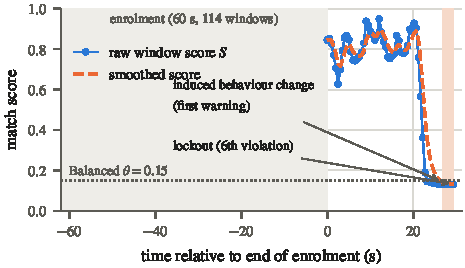
\includegraphics[width=\columnwidth]{figs/field_trace.pdf}
\caption{Team study, session S01 (on-device data). After the 60\,s enrolment the window score stays high; when the author changes their movement it collapses, and the host revokes access six windows after the first warning (shaded).}
\label{fig:trace}
\end{figure}

\subsection{Window-level error: simulation versus headset}
Table~\ref{tab:main} and Fig.~\ref{fig:det} compare error rates. The idealised simulation reaches 2.0\% within a session and 4.7\% across sessions (95\% CI 3.3--6.3\%; AUC 0.989), below the 5\% target. The headset data do not. Counting only different authors as impostors, the EER with interleaved blocks is 17.2\% (AUC 0.909), and averaging scores over 5\,s lowers it to 12.8\%. When the test windows come from the end of the session, as they always do in use, the EER is 30.3\% (95\% CI 16.4--37.5\% from a bootstrap over authors; AUC 0.754), and the deployed full template gives 24.7\%. Per-session EERs under protocol A range from 7.8\% to 62.5\%. Fig.~\ref{fig:matrix} shows why: several templates accept sessions of other authors almost as readily as their own, and a few templates are broad enough to accept most sessions.

\textbf{Deliberate change acts as a disguise.} Each author recorded two or three sessions while deliberately moving differently. Scored against an author's template, that same author's other sessions reached a mean of 0.168, no higher than sessions by other authors (0.171) and far below the session's own held-out windows (0.433). If an author's other sessions are counted as genuine, the person-level EER is 42.7\%, close to chance. Posture explains much of this. Mean eye height per session ranged from 1.06 to 1.56\,m: three of the four authors recorded both seated sessions (1.06--1.22\,m) and standing sessions (1.36--1.56\,m), while three authors standing were within 1\,cm of each other (1.55--1.56\,m). A change of posture therefore moved a person's geometry further than the difference between people. Among the six same-author pairs recorded in a similar posture (eye heights within 10\,cm), the same author scored somewhat higher than other authors in the same posture (mean 0.36 vs.\ 0.29), but six pairs are too few to conclude that the verifier recognises a body. What the data do show is that the verifier detects departures from the behaviour and posture it has just learnt: this is useful against a handover, but a genuine user who sits down or changes task looks like an impostor, and whether an impostor of similar height who adopted the enrolled posture would be caught remains untested. Users of clearly different heights, as expected at an exhibition, are needed to test identification by body geometry.

\begin{table}[t]
\caption{Window-level verification error. Simulation rows are synthetic; headset rows are from on-device logs of 11 sessions by 4 authors, with impostors restricted to different authors (440 genuine, 3,600 impostor windows for A).}
\label{tab:main}
\centering\footnotesize
\setlength{\tabcolsep}{4pt}
\resizebox{\columnwidth}{!}{\begin{tabular}{@{}llcc@{}}
\toprule
Condition & Data & EER & AUC\\
\midrule
Same-session & idealised sim., $N{=}40$ & 2.0\% & --\\
Cross-session & idealised sim., $N{=}40$ & 4.7\% [3.3, 6.3] & 0.989\\
\midrule
Interleaved blocks (C) & headset, 4 authors & 17.2\% & 0.909\\
Interleaved, 5\,s score averaging & headset, 4 authors & 12.8\% & --\\
Deployed template, post-enrolment (B) & headset, 4 authors & 24.7\% & 0.798\\
Held-out end of session (A) & headset, 4 authors & 30.3\% [16.4, 37.5] & 0.754\\
\quad geometry features only & headset, 4 authors & 20.7\% & 0.880\\
\quad dynamics features only & headset, 4 authors & 48.0\% & --\\
\midrule
Held-out end (A), 3 fits, new seed & re-calibrated sim., $N{=}40$ & 28.2--31.4\% & --\\
\bottomrule
\end{tabular}}
\end{table}

\begin{figure}[t]
\centering
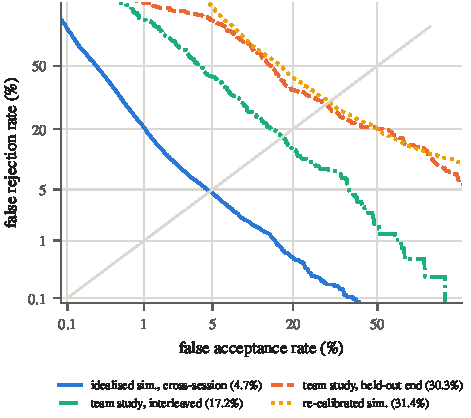
\includegraphics[width=\columnwidth]{figs/det2.pdf}
\caption{Detection error trade-off for the idealised simulation (cross-session), the team study under two protocols, and the re-calibrated simulation.}
\label{fig:det}
\end{figure}

\begin{figure}[t]
\centering
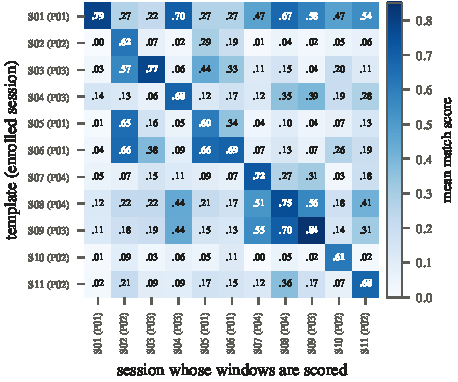
\includegraphics[width=\columnwidth]{figs/field_matrix.pdf}
\caption{Team study: mean score of each session's late enrolment windows against each session's template (built from the first part). Diagonal entries are genuine; labels give session and author. Sessions in chronological order.}
\label{fig:matrix}
\end{figure}

The feature groups explain most of the gap (Fig.~\ref{fig:groups}). In simulation, motion dynamics are as discriminative as geometry (9.1\% vs.\ 10.6\%). In our sessions, dynamics alone were near chance (48.0\%), while geometry alone (20.7\%) beat all 16 features together. Because the authors varied their movement on purpose, this does not show that dynamics carry no identity in natural use; it shows that they are easy to change and should not be relied on. Geometry is harder to change, except through posture, which our authors did change.

\begin{figure}[t]
\centering
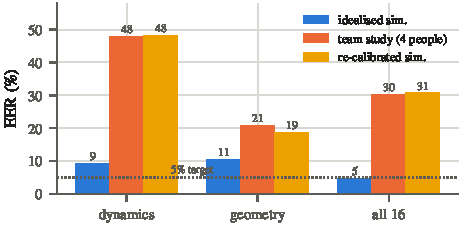
\includegraphics[width=\columnwidth]{figs/groups.pdf}
\caption{EER by feature group (protocol A for the team study and the re-calibrated simulation, cross-session for the idealised simulation).}
\label{fig:groups}
\end{figure}

\subsection{Operating points}
Table~\ref{tab:op} reports stream-level behaviour for the three presets. In the idealised simulation, Strict detects every handover in 2.6\,s but falsely locks out 65\% of genuine two-minute sessions, while Relaxed removes false lockouts and still detects 95\% in 6.1\,s; this result motivated the presets. The headset replay is far less favourable: even Relaxed falsely locks out 4 of 11 genuine 20\,s streams and detects only 47\% of eligible handovers. Scoring only the geometry features improves every preset; with Relaxed it halves the false lockouts to 2 of 11 and detects 78\% of handovers in 5.3\,s on average. The re-calibrated simulation, which was fitted only to window-level EERs, reproduces the headset replay closely: false lockouts of 57--68\%, 25--40\% and 10--28\% of genuine streams and detection rates of 75--93\%, 62--75\% and 47--55\% for Strict, Balanced and Relaxed, against 73\%, 36\%, 36\% and 88\%, 60\%, 47\% on the headset. We take this agreement as evidence that the re-calibrated model captures what matters about the observed behaviour.

\begin{table}[t]
\caption{Operating presets. FL: genuine streams with a false lockout; Det.: detected handovers among those not preceded by a false lockout; Lat.: mean latency after the switch.}
\label{tab:op}
\centering\footnotesize
\setlength{\tabcolsep}{2.5pt}
\resizebox{\columnwidth}{!}{\begin{tabular}{@{}lccc@{}}
\toprule
Preset $(\theta,k)$ & Idealised sim.\ (2\,min streams) & Headset replay, 16 feat.\ (20\,s) & Headset replay, geometry (20\,s)\\
 & FL / Det. / Lat. & FL / Det. / Lat. & FL / Det. / Lat.\\
\midrule
Strict (0.25, 4) & 65\% / 100\% / 2.6\,s & 8/11 / 22/25 / 5.6\,s & 5/11 / 41/48 / 3.8\,s\\
Balanced (0.15, 6) & 18\% / 98\% / 4.3\,s & 4/11 / 35/58 / 5.7\,s & 4/11 / 47/57 / 4.3\,s\\
Relaxed (0.10, 8) & 0\% / 95\% / 6.1\,s & 4/11 / 27/58 / 7.3\,s & 2/11 / 57/73 / 5.3\,s\\
\bottomrule
\end{tabular}}
\end{table}

\subsection{What would it take to reach 5\%?}
We used the re-calibrated simulator to test remedies that we could not test on 11 sessions (Fig.~\ref{fig:remedies}). Longer enrolment helps a little: with all features the EER falls from 27.4\% at 60\,s to 23.0\% at 180\,s (means over the three fits). Geometry-only scoring helps more (18.5\% at 60\,s), and adding 5\,s score averaging gives 16.6\% at 60\,s and 14.6\% at 180\,s (range 12.1--16.3\%). No combination we tested approaches 5\% under the drift we observed. The idealised simulation's 4.7\% therefore depends on assumptions (stationary behaviour, large differences in motion style between people) that our headset data contradict.

\begin{figure}[t]
\centering
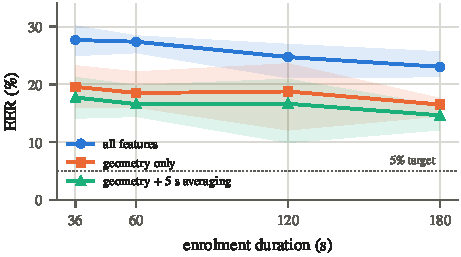
\includegraphics[width=\columnwidth]{figs/remedies.pdf}
\caption{Re-calibrated simulation ($N{=}40$): EER against enrolment duration for three scorers. Lines: mean of the three best fits; bands: their range.}
\label{fig:remedies}
\end{figure}

\section{Discussion}
\textbf{Answer to the research question.} Continuous kinematic verification reached a 4.7\% EER only on idealised simulated users. On a standalone headset, with 60\,s enrolments of free behaviour by four people, the same algorithm separated different people with an EER of 17.2--30.3\%, and a simulator calibrated to these sessions predicts that design changes within this approach stop at about 15\%. A sub-5\% EER for free-use kinematics is not supported by our evidence, although with four people this evidence is preliminary. The system is nevertheless useful as a \emph{second layer}: it caught every induced behaviour change within seconds, and together with the entry gate, which rejected every attempt on another person's gesture, it turns a silent handover into a visible event.

\textbf{Simulation needs a reality check.} Our idealised simulator was calibrated to feature \emph{ranges} from the pilot and passed an independent check (the legacy detector's failure rate). It still overestimated accuracy six-fold, because ranges say nothing about how behaviour drifts within a session or how much motion styles overlap. Matching our headset data required both. We recommend that simulation-based biometric studies report which field statistics their model was fitted to and validate it on a statistic it was not fitted to, as we did with the lockout replay.

\textbf{Geometry over dynamics.} The most actionable finding is that, in our sessions, the useful signal sat in body geometry, while motion dynamics could be changed at will; posture (seated or standing) should be detected and enrolled separately rather than treated as an anomaly. Structured motion is different: the gesture factor, a short deliberate stroke, separated owners from non-owners perfectly in our small sample. Asking for occasional short, structured motions (``task-anchored'' verification) and weighting geometry when nothing structured is happening are promising directions.

\textbf{A detector that cannot tell people apart should not revoke them.} The speed-threshold detector failed the same way in both studies, revoking almost every genuine session within about 10\,s. Identity decisions should rest on an enrolled template; transient anomaly signals should at most raise a warning.

\textbf{Error rate is not user experience.} Window-level EER does not predict lockouts: because windows overlap, low scores come in runs, and the choice of $(\theta, k)$ moves false lockouts between 0\% and 65\% in simulation at the same EER. Evaluations of continuous authentication should report stream-level false-lockout and detection-latency figures, measured on headset data where possible.

\section{Limitations and Ethics}
The headset study is small and not independent: the four authors produced all 11 sessions on one day and one headset, and they deliberately varied their behaviour between sessions to stand in for different users. This role-play is not the same as independent users, it does not meet the usual requirement of at least ten participants, and the confidence intervals are correspondingly wide. Genuine test data come from the same session as enrolment; cross-day effects, which are known to be large~\cite{miller2022}, are only simulated. Lockouts were induced by authors who knew the system was watching their movement, so the 9 of 9 detection rate is an upper bound for real handovers. Window-level splicing in the handover replay omits the windows that straddle a real switch. The re-calibrated simulator matches our data by construction on four statistics and is non-identifiable; we therefore report the range over three fits and treat its remedy predictions as indicative. Mimicry was not evaluated. No data from people outside the team were used; motion data are themselves identifying~\cite{miller2020,nair2023}, so templates stay on the device. A study with independent participants, multiple days and a formal consent protocol is the priority for future work and is planned at the project exhibition.

\section{Conclusion}
We built a VR boardroom that verifies its wearer continuously after a three-factor login and evaluated it in simulation and on a standalone headset. In use, it behaved as intended: the entry gate stopped people without the owner's gesture, and the verifier locked out every deliberate behaviour change within seconds. Its accuracy, however, was far below what an idealised simulation predicted: 17.2--30.3\% EER between the four authors against 4.7\% in simulation. A simulator re-calibrated to the headset data explains the gap (behaviour drifts within a session, and motion styles overlap) and reproduces the observed lockout rates without being fitted to them. Body geometry was the more useful signal, but a change between sitting and standing moved it further than the difference between people, so the same person could look like someone else. We release the code, the on-device logs and both simulators so that others can test these conclusions with independent participants.

\section*{Acknowledgment}
Generative AI (Anthropic Claude) was used to assist with software implementation, data analysis and drafting of this manuscript, as disclosed in Section~5.1 of the project dossier. The authors reviewed and take responsibility for all content.

\begin{thebibliography}{99}\footnotesize
\bibitem{pfeuffer2019} K.~Pfeuffer, M.~J.~Geiger, S.~Prange, L.~Mecke, D.~Buschek, and F.~Alt, ``Behavioural biometrics in VR: Identifying people from body motion and relations in virtual reality,'' in \emph{Proc. CHI Conf. Human Factors in Computing Systems (CHI)}, 2019, pp.~1--12, doi: 10.1145/3290605.3300340.
\bibitem{miller2020} M.~R.~Miller, F.~Herrera, H.~Jun, J.~A.~Landay, and J.~N.~Bailenson, ``Personal identifiability of user tracking data during observation of 360-degree VR video,'' \emph{Scientific Reports}, vol.~10, art.~17404, 2020, doi: 10.1038/s41598-020-74486-y.
\bibitem{nair2023} V.~Nair, W.~Guo, J.~Mattern, R.~Wang, J.~F.~O'Brien, L.~Rosenberg, and D.~Song, ``Unique identification of 50,000+ virtual reality users from head \& hand motion data,'' in \emph{Proc. 32nd USENIX Security Symp.}, 2023.
\bibitem{mustafa2018} T.~Mustafa, R.~Matovu, A.~Serwadda, and N.~Muirhead, ``Unsure how to authenticate on your VR headset? Come on, use your head!'' in \emph{Proc. 4th ACM Int. Workshop on Security and Privacy Analytics (IWSPA)}, 2018, pp.~23--30, doi: 10.1145/3180445.3180450.
\bibitem{gyreyiri2025} P.~S.~Gyreyiri and D.~Shukla, ``Head movement biometrics for continuous authentication in virtual reality,'' in \emph{Proc. 31st ACM Symp. Virtual Reality Software and Technology (VRST)}, 2025, doi: 10.1145/3756884.3768408.
\bibitem{george2017} C.~George, M.~Khamis, E.~von Zezschwitz, H.~Schmidt, M.~Burger, F.~Alt, and H.~Hussmann, ``Seamless and secure VR: Adapting and evaluating established authentication systems for virtual reality,'' in \emph{Proc. Workshop on Usable Security (USEC)}, 2017, doi: 10.14722/usec.2017.23028.
\bibitem{stephenson2022} S.~Stephenson, B.~Pal, S.~Fan, E.~Fernandes, Y.~Zhao, and R.~Chatterjee, ``SoK: Authentication in augmented and virtual reality,'' in \emph{Proc. IEEE Symp. Security and Privacy (SP)}, 2022, pp.~267--284, doi: 10.1109/SP46214.2022.9833742.
\bibitem{li2016} S.~Li, A.~Ashok, Y.~Zhang, C.~Xu, J.~Lindqvist, and M.~Gruteser, ``Whose move is it anyway? Authenticating smart wearable devices using unique head movement patterns,'' in \emph{Proc. IEEE Int. Conf. Pervasive Computing and Communications (PerCom)}, 2016, pp.~1--9, doi: 10.1109/PERCOM.2016.7456514.
\bibitem{miller2022} R.~Miller, N.~K.~Banerjee, and S.~Banerjee, ``Temporal effects in motion behavior for virtual reality (VR) biometrics,'' in \emph{Proc. IEEE Conf. Virtual Reality and 3D User Interfaces (VR)}, 2022, pp.~563--572, doi: 10.1109/VR51125.2022.00076.
\bibitem{chen2024} F.~Chen, J.~Xin, and V.~V.~Phoha, ``SSPRA: A robust approach to continuous authentication amidst real-world adversarial challenges,'' \emph{IEEE Trans. Biometrics, Behavior, and Identity Science}, vol.~6, no.~2, pp.~245--260, 2024, doi: 10.1109/TBIOM.2024.3369590.
\bibitem{li2026} M.~Li, N.~K.~Banerjee, and S.~Banerjee, ``Real or fake motion: Protecting virtual reality (VR) behavioral authentication systems against motion forecasting attacks,'' \emph{Frontiers in Virtual Reality}, vol.~7, 2026, doi: 10.3389/frvir.2026.1766672.
\end{thebibliography}
